% Section 1 - Sensor sampling
% Roberto Masocco <roberto.masocco@uniroma2.it>
% May 28, 2024

% ### Sensor sampling ###
\section{Sensor sampling}
\graphicspath{{figs/section1/}}

% --- Sensor sampling basics ---
\begin{frame}{Sensor sampling basics}{From theory to practice}
	\begin{columns}
		\column{.5\textwidth}
		\textbg{Sampling} a sensor consists of reading \textbg{measurements} from it, to be fed to a control loop or some other subsystem.\\
    It requires:
		\begin{itemize}
			\item the definition of a \textbg{sampling frequency};
			\item the implementation of an \textbg{encoding};
			\item the application of \textbg{post-processing} steps (\emph{e.g.}, \textbg{filtering}).
		\end{itemize}

		\column{.5\textwidth}
		\begin{figure}
			\centering
			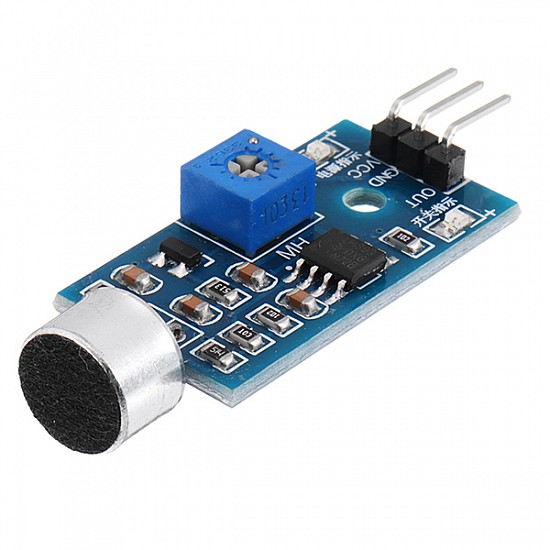
\includegraphics[width=.7\textwidth]{sensor.jpeg}
			\caption{Analog sound sensor.}
			\label{fig:sensor}
		\end{figure}
	\end{columns}
\end{frame}

% --- Sensor sampling with ROS 2 ---
\begin{frame}{Sensor sampling with ROS 2}{Driver modules}
	Sampling is generally handled by \textbg{microcontrollers}, but when the sampling frequency is not too high, \emph{e.g.}, down to some ms, it can be carried out by a higher-level device.\\
	To implement a ROS 2 sensor sampling module, one has to develop a \textbg{driver node}, \emph{i.e.}, an application that:
	\begin{itemize}
		\item configures the \textbg{sensor hardware} to run as required;
		\item ensures \textbg{stable sampling frequency} and \textbg{low jitter};
		\item outputs data with a \textbg{standard interface} and \textbg{low latency}.
	\end{itemize}
  The achievement of the first goal depends on the \textbg{sensor}, the second on the \textbg{system} (hardware and software!), while the third one is solved by ROS 2 (\textbg{messages}, \textbg{QoS}).
	\begin{block}{}
		\centering
		\textbf{Must take the best of both worlds: robotics and system programming!}
	\end{block}
\end{frame}

% --- Anatomy of a driver node ---
\begin{frame}{Anatomy of a driver node}{Guidelines and best practices}
  In essence, a \textbg{driver node} always consists of:
  \begin{itemize}
    \item an \textbg{enable service}, to be called to start or stop the sampling;
    \item a \textbg{hardware configuration} routine, to be run at startup or when enabled;
    \item a \textbg{sampling loop}, to be run at a fixed frequency in a separate \textbg{thread};
    \item a \textbg{publisher} using a common message type and an appropriate QoS policy;
    \item a set of \textbg{parameters} to configure the sensor and the sampling loop;
    \item \textbg{launch files} and \textbg{configuration files}, to configure remapping rules and node behaviour.
  \end{itemize}
\end{frame}
